\experiment{Graph adjacency matrix method}{29/11/2023}

\section{Aim}
Write a C Program to represent any given graph and to do the following operations:
\\1. Compute adjacency matrix
\\2. Perform a depth first search
\\3. Perform a breadth first search

\section{Algorithm}
 {\fontfamily{lmtt}\selectfont
  \subsection{Main Function}
  \begin{enumerate}[label=\arabic*:,left=0pt]
    \item \textbf{Start}
    \item Create a \texttt{graph} pointer \texttt{g} and set it to \texttt{createGraph(20)}.
    \item Print the graph structure.
    \item Insert edges to create the following graph structure:
          \begin{itemize}
            \item \(1 - 2 - 4 - 6 - 8 - 10\)
            \item \(|\)
            \item \(3 - 5 - 7 - 9\)
          \end{itemize}
    \item Display the graph.
    \item Call \texttt{dfs(g, 2)} to perform Depth-First Search starting from node 2.
    \item Call \texttt{bfs(g, 2)} to perform Breadth-First Search starting from node 2.
    \item \textbf{Stop}
  \end{enumerate}

  \subsection{\texttt{createGraph(size)}}
  \begin{enumerate}[label=\arabic*:,left=0pt]
    \item \textbf{Start}
    \item Allocate memory for a \texttt{graph} structure \texttt{g}.
    \item Set \texttt{g->v} to \texttt{size}.
    \item Set \texttt{g->e} to 0.
    \item Allocate memory for the adjacency matrix \texttt{g->matrix} with dimensions \texttt{(size + 1) by (size + 1)}.
    \item Initialize all elements of \texttt{g->matrix} to 0.
    \item Return \texttt{g}.
    \item \textbf{Stop}
  \end{enumerate}

  \subsection{\texttt{insertEdge(g, from, to)}}
  \begin{enumerate}[label=\arabic*:,left=0pt]
    \item \textbf{Start}
    \item Allocate memory for a new \texttt{edge} structure \texttt{new}.
    \item If \texttt{from} or \texttt{to} is greater than \texttt{g->v}, print "Edge not valid!!" and return.
    \item Set \texttt{g->matrix[from][to]} to 1.
    \item Increment \texttt{g->e}.
    \item \textbf{Stop}
  \end{enumerate}

  \subsection{\texttt{display(g)}}
  \begin{enumerate}[label=\arabic*:,left=0pt]
    \item \textbf{Start}
    \item Print "Nodes = \texttt{g->v}, Edges = \texttt{g->e}".
    \item Loop over \texttt{i} from 0 to \texttt{g->v}:
          \begin{enumerate}[label=2.\arabic*:, start=1]
            \item Print "\texttt{i : }".
            \item Loop over \texttt{j} from 0 to \texttt{g->v}:
                  \begin{enumerate}[label=2.2.\arabic*:, start=1]
                    \item If \texttt{g->matrix[i][j] == 1}, print "\texttt{j}".
                  \end{enumerate}
            \item Print a newline.
          \end{enumerate}
    \item \textbf{Stop}
  \end{enumerate}

  \subsection{\texttt{dfs(g, start)}}
  \begin{enumerate}[label=\arabic*:,left=0pt]
    \item \textbf{Start}
    \item Print "DFS".
    \item Create a \texttt{stack}\ \texttt{s}
    \item Allocate memory for an array \texttt{visited} of size \texttt{g->v + 1} and initialize all elements to 0.
    \item If \texttt{start > g->v}, print "Not a valid node!!" and return.
    \item Push \texttt{start} onto the stack.
    \item While \texttt{s->top != -1}:
          \begin{enumerate}[label=7.\arabic*:, start=1]
            \item Set \texttt{node} to the element at the top of the stack.
            \item If \texttt{!visited[node]}, print "\texttt{node , }".
            \item Set \texttt{visited[node]} to 1.
            \item Set \texttt{flag} to 0.
            \item Loop over \texttt{i} from 0 to \texttt{g->v}:
                  \begin{enumerate}[label=7.5.\arabic*:, start=1]
                    \item If \texttt{g->matrix[node][i] != 0} and \texttt{!visited[i]}, push \texttt{i} onto the stack, set \texttt{flag} to 1,\newline and break.
                  \end{enumerate}
            \item If \texttt{!flag}, pop the stack.
          \end{enumerate}
    \item Free \texttt{visited}
    \item Print a newline.
    \item \textbf{Stop}
  \end{enumerate}

  \subsection{\texttt{bfs(g, start)}}
  \begin{enumerate}[label=\arabic*:,left=0pt]
    \item \textbf{Start}
    \item Print "BFS".
    \item Create a \texttt{queue} \ \texttt{q}
    \item Allocate memory for an array \texttt{visited} of size \texttt{g->v + 1} and initialize all elements to 0.
    \item If \texttt{start > g->v}, print "Not a valid node!!" and return.
    \item Enqueue \texttt{start} into the queue.
    \item While \texttt{q->front != -1}:
          \begin{enumerate}[label=7.\arabic*:, start=1]
            \item Set \texttt{node} to the element dequeued from the queue.
            \item If \texttt{visited[node]}, continue to the next iteration.
            \item Set \texttt{visited[node]} to 1.
            \item Print "\texttt{node , }".
            \item Loop over \texttt{i} from 0 to \texttt{g->v}:
                  \begin{enumerate}[label=7.5.\arabic*:, start=1]
                    \item If \texttt{g->matrix[node][i] != 0}, enqueue \texttt{i} into the queue.
                  \end{enumerate}
          \end{enumerate}
    \item Free \texttt{q} and \texttt{visited}.
    \item Print a newline.
    \item \textbf{Stop}
  \end{enumerate}
 }

\section{C Program}

\begin{lstlisting}[label={list:c_progam1:graph-GraphAdjMatrix}]
#include <stdio.h>
#include <stdlib.h>

// Graph
typedef struct Edge
{
  int from;
  int to;
} edge;
typedef struct Graph
{
  int v;
  int e;
  int **matrix;
} graph;

graph *createGraph(int size);
void insertEdge(graph *g, int from, int to);
void display(graph *g);
void dfs(graph *g, int start);
void bfs(graph *g, int start);

// Stack
typedef struct Stack
{
  int top;
  int size;
  int arr[100];
} stack;

stack *createStack();
void push(stack *s, int data);
int pop(stack *s);
void tos(stack *s);

// Queue
typedef struct queue
{
  int front;
  int back;
  int size;
  int arr[100];
} queue;

queue *createQueue();
void enqueue(queue *q, int data);
int dequeue(queue *q);

int main()
{
  graph *g = createGraph(20);

  /*
    1 - 2 - 4 - 6 - 8 - 10
    |
    3 - 5 - 7 - 9
  */

  insertEdge(g, 1, 2);
  insertEdge(g, 1, 3);
  insertEdge(g, 2, 1);
  insertEdge(g, 2, 4);
  insertEdge(g, 3, 5);
  insertEdge(g, 4, 6);
  insertEdge(g, 5, 7);
  insertEdge(g, 6, 8);
  insertEdge(g, 7, 9);
  insertEdge(g, 8, 9);
  insertEdge(g, 8, 10);
  display(g);
  dfs(g, 2);
  bfs(g, 2);
}

graph *createGraph(int size)
{
  graph *g = (graph *)malloc(sizeof(graph));
  g->v = size;
  g->e = 0;
  g->matrix = (int **)malloc(sizeof(int *) * (size + 1));
  for (int i = 0; i <= size; i++)
  {
    g->matrix[i] = (int *)malloc(sizeof(int) * (size + 1));
    for (int j = 0; j <= size; j++)
    {
      g->matrix[i][j] = 0;
    }
  }
  return g;
}

void insertEdge(graph *g, int from, int to)
{
  edge *new = (edge *)malloc(sizeof(edge));

  if (from > g->v || to > g->v)
  {
    printf("Edge doesn't exist!!\n");
    return;
  }
  g->matrix[from][to] = 1;
  g->e++;
}

void display(graph *g)
{
  printf("Nodes = %d, Edges = %d\n", g->v, g->e);
  for (int i = 0; i <= g->v; i++)
  {
    printf("%d : ", i);
    for (int j = 0; j <= g->v; j++)
    {
      if (g->matrix[i][j] == 1)
      {
        printf("%d ", j);
      }
    }
    printf("\n");
  }
}

void dfs(graph *g, int start)
{
  printf("DFS\n");
  stack *s = createStack();
  int *visited = calloc(g->v + 1, sizeof(int));
  if (start > g->v)
  {
    printf("Not a valid node!!\n");
    return;
  }
  push(s, start);
  while (s->top != -1)
  {
    int node = s->arr[s->top];
    if (!visited[node])
    {
      printf("%d , ", node);
    }
    visited[node] = 1;
    int flag = 0;
    for (int i = 0; i <= g->v; i++)
    {
      if (g->matrix[node][i] != 0 && !visited[i])
      {
        push(s, i);
        flag = 1;
        break;
      }
    }
    if (!flag)
    {
      pop(s);
    }
  }
  free(visited);
  free(s);
  printf("\n");
}

void bfs(graph *g, int start)
{
  printf("BFS\n");
  queue *q = createQueue();
  int *visited = calloc(g->v + 1, sizeof(int));
  if (start > g->v)
  {
    printf("Not a valid node!!\n");
    return;
  }
  enqueue(q, start);
  while (q->front != -1)
  {
    int node = dequeue(q);
    if (visited[node])
    {
      continue;
    }
    visited[node] = 1;
    printf("%d , ", node);
    for (int i = 0; i <= g->v; i++)
    {
      if (g->matrix[node][i] != 0)
      {
        enqueue(q, i);
      }
    }
  }
  free(q);
  free(visited);
  printf("\n");
}
stack *createStack()
{
  stack *s = (stack *)malloc(sizeof(stack));
  s->top = -1;
  s->size = 100;
  return s;
}

void push(stack *s, int data)
{
  // printf("Pushed - %d\n ", data);
  if (s->top == s->size - 1)
  {
    printf("Stack Overflow\n");
    return;
  }
  s->top++;
  s->arr[s->top] = data;
}

int pop(stack *s)
{
  if (s->top < 0)
  {
    printf("Stack underflow\n");
    return -1;
  }
  s->top--;
  return s->arr[s->top + 1];
}

queue *createQueue()
{
  queue *q = (queue *)malloc(sizeof(queue));
  q->front = -1;
  q->back = -1;
  q->size = 100;
  return q;
}

void enqueue(queue *q, int data)
{
  if (q->front == -1 && q->back == -1)
  {
    q->front = 0;
    q->back = 0;
    q->arr[q->back] = data;
    return;
  }
  else if (q->back == q->size - 1)
  {
    printf("\nQueue overflow\n");
    return;
  }
  q->back++;
  q->arr[q->back] = data;
}

int dequeue(queue *q)
{
  int removed;
  if (q->back == q->front)
  {
    if (q->front == -1)
    {
      printf("\nQueue underflow!\n");
      return -1;
    }
    removed = q->arr[q->front];
    q->front = -1;
    q->back = -1;
  }
  else
  {
    removed = q->arr[q->front];
    q->front++;
  }
  q->size--;
  return removed;
}

\end{lstlisting}


\section{Output}
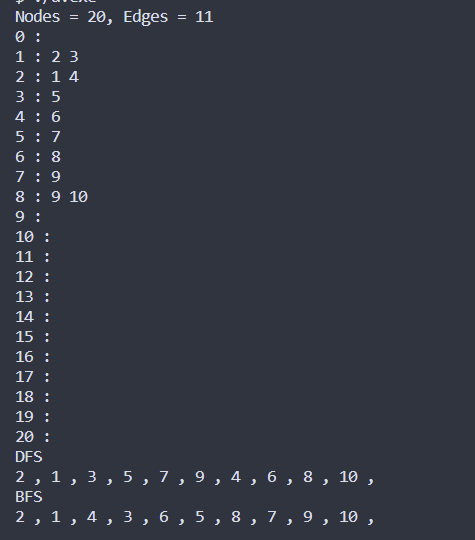
\includegraphics[]{Cycle_2/Outputs/GraphAdjMatrix.png}

\section{Result}
Graph representations and traversals implemented. The program was executed and output
verified.